\documentclass{ximera}

%\usepackage{todonotes}

\newcommand{\todo}{}

\usepackage{tkz-euclide}
\tikzset{>=stealth} %% cool arrow head
\tikzset{shorten <>/.style={ shorten >=#1, shorten <=#1 } } %% allows shorter vectors

\usepackage{tkz-tab}  %% sign charts
\usetikzlibrary{decorations.pathreplacing} 

\usetikzlibrary{backgrounds} %% for boxes around graphs
\usetikzlibrary{shapes,positioning}  %% Clouds and stars
\usetikzlibrary{matrix} %% for matrix
\usepgfplotslibrary{polar} %% for polar plots
\usetkzobj{all}
\usepackage[makeroom]{cancel} %% for strike outs
%\usepackage{mathtools} %% for pretty underbrace % Breaks Ximera
\usepackage{multicol}

\usepackage{polynom}



\usepackage[many]{tcolorbox}  %% for titled boxes
\newtcolorbox{xbox}[1]{%
    tikznode boxed title,
    enhanced,
    arc=0mm,
    interior style={white},
    attach boxed title to top center= {yshift=-\tcboxedtitleheight/2},
    fonttitle=\bfseries,
    colbacktitle=white,coltitle=black,
    boxed title style={size=normal,colframe=white,boxrule=0pt},
    title={#1}}


\usepackage{array}
\setlength{\extrarowheight}{+.1cm}   
\newdimen\digitwidth
\settowidth\digitwidth{9}
\def\divrule#1#2{
\noalign{\moveright#1\digitwidth
\vbox{\hrule width#2\digitwidth}}}





\newcommand{\RR}{\mathbb R}
\newcommand{\R}{\mathbb R}
\newcommand{\N}{\mathbb N}
\newcommand{\Z}{\mathbb Z}

%\renewcommand{\d}{\,d\!}
\renewcommand{\d}{\mathop{}\!d}
\newcommand{\dd}[2][]{\frac{\d #1}{\d #2}}
\newcommand{\pp}[2][]{\frac{\partial #1}{\partial #2}}
\renewcommand{\l}{\ell}
\newcommand{\ddx}{\frac{d}{\d x}}
\newcommand{\ddt}{\frac{d}{\d t}}

\newcommand{\zeroOverZero}{\ensuremath{\boldsymbol{\tfrac{0}{0}}}}
\newcommand{\inftyOverInfty}{\ensuremath{\boldsymbol{\tfrac{\infty}{\infty}}}}
\newcommand{\zeroOverInfty}{\ensuremath{\boldsymbol{\tfrac{0}{\infty}}}}
\newcommand{\zeroTimesInfty}{\ensuremath{\small\boldsymbol{0\cdot \infty}}}
\newcommand{\inftyMinusInfty}{\ensuremath{\small\boldsymbol{\infty - \infty}}}
\newcommand{\oneToInfty}{\ensuremath{\boldsymbol{1^\infty}}}
\newcommand{\zeroToZero}{\ensuremath{\boldsymbol{0^0}}}
\newcommand{\inftyToZero}{\ensuremath{\boldsymbol{\infty^0}}}



\newcommand{\numOverZero}{\ensuremath{\boldsymbol{\tfrac{\#}{0}}}}
\newcommand{\dfn}{\textbf}
%\newcommand{\unit}{\,\mathrm}
\newcommand{\unit}{\mathop{}\!\mathrm}
\newcommand{\eval}[1]{\bigg[ #1 \bigg]}
\newcommand{\seq}[1]{\left( #1 \right)}
\renewcommand{\epsilon}{\varepsilon}
\renewcommand{\iff}{\Leftrightarrow}

\DeclareMathOperator{\arccot}{arccot}
\DeclareMathOperator{\arcsec}{arcsec}
\DeclareMathOperator{\arccsc}{arccsc}
\DeclareMathOperator{\si}{Si}
\DeclareMathOperator{\proj}{proj}
\DeclareMathOperator{\scal}{scal}


\newcommand{\tightoverset}[2]{% for arrow vec
  \mathop{#2}\limits^{\vbox to -.5ex{\kern-0.75ex\hbox{$#1$}\vss}}}
\newcommand{\arrowvec}[1]{\tightoverset{\scriptstyle\rightharpoonup}{#1}}
\renewcommand{\vec}{\mathbf}
\newcommand{\veci}{\vec{i}}
\newcommand{\vecj}{\vec{j}}
\newcommand{\veck}{\vec{k}}
\newcommand{\vecl}{\boldsymbol{\l}}

\newcommand{\dotp}{\bullet}
\newcommand{\cross}{\boldsymbol\times}
\newcommand{\grad}{\boldsymbol\nabla}
\newcommand{\divergence}{\grad\dotp}
\newcommand{\curl}{\grad\cross}
%\DeclareMathOperator{\divergence}{divergence}
%\DeclareMathOperator{\curl}[1]{\grad\cross #1}


\colorlet{textColor}{black} 
\colorlet{background}{white}
\colorlet{penColor}{blue!50!black} % Color of a curve in a plot
\colorlet{penColor2}{red!50!black}% Color of a curve in a plot
\colorlet{penColor3}{red!50!blue} % Color of a curve in a plot
\colorlet{penColor4}{green!50!black} % Color of a curve in a plot
\colorlet{penColor5}{orange!80!black} % Color of a curve in a plot
\colorlet{fill1}{penColor!20} % Color of fill in a plot
\colorlet{fill2}{penColor2!20} % Color of fill in a plot
\colorlet{fillp}{fill1} % Color of positive area
\colorlet{filln}{penColor2!20} % Color of negative area
\colorlet{fill3}{penColor3!20} % Fill
\colorlet{fill4}{penColor4!20} % Fill
\colorlet{fill5}{penColor5!20} % Fill
\colorlet{gridColor}{gray!50} % Color of grid in a plot

\newcommand{\surfaceColor}{violet}
\newcommand{\surfaceColorTwo}{redyellow}
\newcommand{\sliceColor}{greenyellow}




\pgfmathdeclarefunction{gauss}{2}{% gives gaussian
  \pgfmathparse{1/(#2*sqrt(2*pi))*exp(-((x-#1)^2)/(2*#2^2))}%
}


%%%%%%%%%%%%%
%% Vectors
%%%%%%%%%%%%%

%% Simple horiz vectors
\renewcommand{\vector}[1]{\left\langle #1\right\rangle}


%% %% Complex Horiz Vectors with angle brackets
%% \makeatletter
%% \renewcommand{\vector}[2][ , ]{\left\langle%
%%   \def\nextitem{\def\nextitem{#1}}%
%%   \@for \el:=#2\do{\nextitem\el}\right\rangle%
%% }
%% \makeatother

%% %% Vertical Vectors
%% \def\vector#1{\begin{bmatrix}\vecListA#1,,\end{bmatrix}}
%% \def\vecListA#1,{\if,#1,\else #1\cr \expandafter \vecListA \fi}

%%%%%%%%%%%%%
%% End of vectors
%%%%%%%%%%%%%

%\newcommand{\fullwidth}{}
%\newcommand{\normalwidth}{}



%% makes a snazzy t-chart for evaluating functions
%\newenvironment{tchart}{\rowcolors{2}{}{background!90!textColor}\array}{\endarray}

%%This is to help with formatting on future title pages.
\newenvironment{sectionOutcomes}{}{} 



%% Flowchart stuff
%\tikzstyle{startstop} = [rectangle, rounded corners, minimum width=3cm, minimum height=1cm,text centered, draw=black]
%\tikzstyle{question} = [rectangle, minimum width=3cm, minimum height=1cm, text centered, draw=black]
%\tikzstyle{decision} = [trapezium, trapezium left angle=70, trapezium right angle=110, minimum width=3cm, minimum height=1cm, text centered, draw=black]
%\tikzstyle{question} = [rectangle, rounded corners, minimum width=3cm, minimum height=1cm,text centered, draw=black]
%\tikzstyle{process} = [rectangle, minimum width=3cm, minimum height=1cm, text centered, draw=black]
%\tikzstyle{decision} = [trapezium, trapezium left angle=70, trapezium right angle=110, minimum width=3cm, minimum height=1cm, text centered, draw=black]


\title[Dig-In:]{Inverses of functions}


\outcome{Find the domain and range of a function.}
\outcome{Determine if a function is one-to-one.}
\outcome{Perform basic operations and compositions on functions.}
\outcome{Define and work with inverse functions.}
\outcome{Plot inverses of basic functions.}
\outcome{Find inverse functions (algebraically and graphically).}
\outcome{Find the largest interval containing a given point
  where the function is invertible.}
\outcome{Determine the intervals on which a function has an inverse.}



\begin{document}
\begin{abstract}
  Here we ``undo'' functions.
\end{abstract}
\maketitle


If a function maps every ``input'' to exactly one ``output,'' an
inverse of that function maps every ``output'' to exactly one
``input.''  We need a more formal definition to actually say anything
with rigor.

\begin{definition}
  Let $f$ be a function with domain $A$ and range $B$:
  \begin{image}
    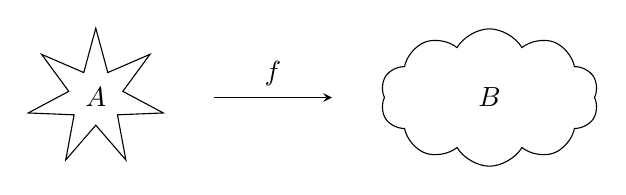
\begin{tikzpicture}
      \node[star,star points=7,star point ratio=2.5,draw] at (0,0) {$A$};
      \node[cloud, draw,cloud puffs=10,cloud puff arc=120, aspect=2, inner ysep=1em] at (5,0) {$B$};
      \node at (2.25,.3) {$f$};
      \draw[->] (1.5,0) to (3,0);
    \end{tikzpicture}
  \end{image}
  Let $g$ be a function with domain $B$ and range $A$:
  \begin{image}
    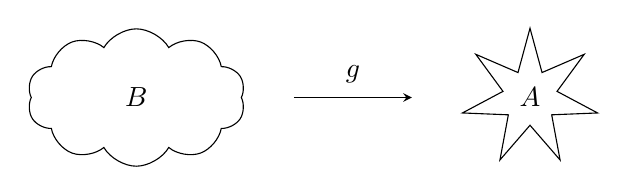
\begin{tikzpicture}
      \node[cloud, draw,cloud puffs=10,cloud puff arc=120, aspect=2, inner ysep=1em] at (-.5,0) {$B$};
      \node[star,star points=7,star point ratio=2.5,draw] at (4.5,0) {$A$};
      \node at (2.25,.3) {$g$};
      \draw[->] (1.5,0) to (3,0);
    \end{tikzpicture}
  \end{image}
  We say that $f$ and $g$ are \dfn{inverses} of each other if $f(g(b))
  = b$ for all $b$ in $B$, and also $g(f(a)) = a$ for all $a$ in $A$.
  Sometimes we write $g = f^{-1}$ in this case.
  \begin{image}
    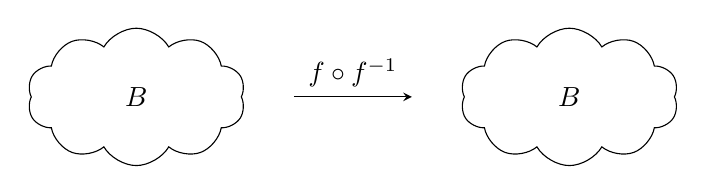
\begin{tikzpicture}
      \node[cloud, draw,cloud puffs=10,cloud puff arc=120, aspect=2, inner ysep=1em] at (-.5,0) {$B$};
      \node[cloud, draw,cloud puffs=10,cloud puff arc=120, aspect=2, inner ysep=1em] at (5,0) {$B$};
      \node at (2.25,.3) {$f\circ f^{-1}$};
      \draw[->] (1.5,0) to (3,0);
    \end{tikzpicture}
  \end{image}
  and
  \begin{image}
    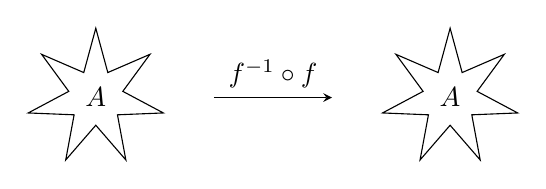
\begin{tikzpicture}
      \node[star,star points=7,star point ratio=2.5,draw] at (0,0) {$A$};
      \node[star,star points=7,star point ratio=2.5,draw] at (4.5,0) {$A$};
      \node at (2.25,.3) {$f^{-1}\circ f$};
      \draw[->] (1.5,0) to (3,0);
    \end{tikzpicture}
  \end{image}
  So, we could rephrase these conditions as
  \[
  f(f^{-1}(x)) = x\qquad\text{and}\qquad f^{-1}(f(x)) = x.
  \]
  \end{definition}
These two simple equations are somewhat more subtle than they
initially appear.

\begin{question}
  Let $f$ be a function.  If the point $(1,9)$ is on the graph of $f$,
  what point must be the the graph of $f^{-1}$?
  \begin{prompt}
  \[
  \left( \answer{9}, \answer{1} \right)
  \]
  \end{prompt}
  \begin{feedback}
    Since $f(1) = 9$, we must have $f^{-1}(f(1)) = 1$, so $f^{-1}(9) =
    1$.  Thus $(9,1)$ is on the graph of $f^{-1}$.  This is a general
    rule.  If $(a,b)$ is on the graph of $f$, then $(b,a)$ will be on the
    graph of $f^{-1}$.
  \end{feedback}
\end{question}

\begin{warning}
  This notation can be very confusing.  Keep a watchful eye:
  \begin{align*}
    f^{-1}(x) &= \text{the inverse function of $f(x)$.}\\
    f(x)^{-1} &= \text{$\frac{1}{f(x)}$.}
  \end{align*}
\end{warning}
\begin{question}
  Which of the following is notation for the inverse of the function
  $\sin(\theta)$ on the interval $[-\pi/2,\pi/2]$?
  \begin{multipleChoice}
    \choice[correct]{$\sin^{-1}(\theta)$}
    \choice{$\sin(\theta)^{-1}$}
  \end{multipleChoice}
  \begin{feedback}
    $\sin^{-1}(\theta)$ is the inverse function for $\sin(\theta)$ on
    the interval $[-\pi/2,\pi/2]$.

    On the other hand,
    \[
    \sin(\theta)^{-1} = \frac{1}{\sin(\theta)} \ne \sin^{-1}(\theta).
    \]
  \end{feedback}
\end{question}


\begin{question}
  Consider the graph of $y=f(x)$ below
  \begin{image}
    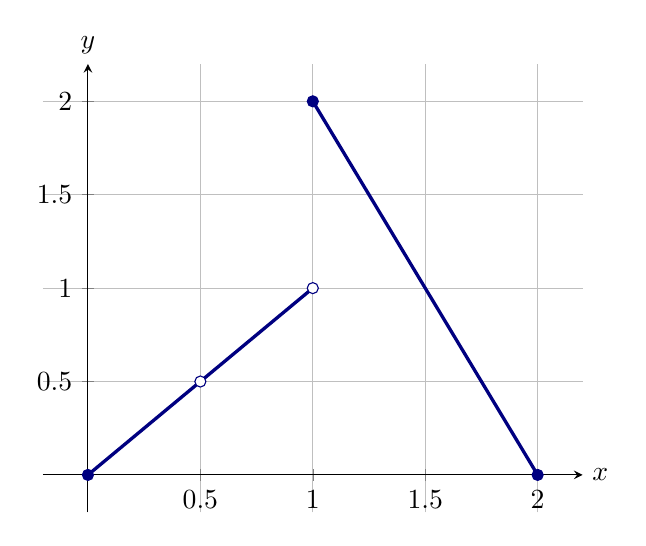
\begin{tikzpicture}
      \begin{axis}
	[xmin=-0.2,
          xmax=2.2,
          ymin=-0.2,
          ymax=2.2,
          axis lines=center,
          xlabel=$x$,ylabel=$y$,
          every axis y label/.style={at=(current axis.above origin),anchor=south},
          every axis x label/.style={at=(current axis.right of origin),anchor=west},
	  domain=-1:2,
          clip=false,
	  ytick={0.5,1,1.5,2},
	  yticklabels={$0.5$,$1$,$1.5$,$2$},
	  xtick={0.5,1.0,1.5,2},
	  xticklabels={$0.5$,$1$,$1.5$,$2$},
	  grid = major
	]
        \addplot[very thick,penColor] plot coordinates {(0,0) (1,1)};
        \addplot[very thick,penColor] plot coordinates {(1,2) (2,0)};
        
        %\draw[very thin,color=black] (axis cs:0,-0.2) -- (axis cs:0,2);

        \addplot[color=penColor,fill=background,only marks,mark=*] coordinates{(1,1)};  %% open hole
        \addplot[color=penColor,fill=background,only marks,mark=*] coordinates{(.5,.5)};  %% open hole

        \addplot[color=penColor,fill=penColor,only marks,mark=*] coordinates{(0,0)};  %% closed hole
        \addplot[color=penColor,fill=penColor,only marks,mark=*] coordinates{(2,0)};  %% closed hole
        \addplot[color=penColor,fill=penColor,only marks,mark=*] coordinates{(1,2)};  %% closed hole
        
        %% \draw[fill=black] (axis cs:0,0) circle [radius=2pt];
	%% \draw[fill=black] (axis cs:2,0) circle [radius=2pt];
        %% \draw[fill=black] (axis cs:1,2) circle [radius=2pt];
	
	\end{axis}
    \end{tikzpicture}
  \end{image}
  Is $f(x)$ invertible at $x=1$?
  \begin{prompt}
  \begin{multipleChoice}
    \choice[correct]{yes}
    \choice{no}
  \end{multipleChoice}
  \begin{question}
    \[
    f^{-1}(1) = \answer{1.5}
    \]
  \end{question}
  \end{prompt}
\end{question}


So far, we've only dealt with abstract examples.  Let's see
if we can ground this in a real-life context.

\begin{example}
  The function
  \[
  f(t) = \left(\frac{9}{5}\right) t + 32
  \]	
  takes a temperature $t$ in degrees Celsius, and converts it into Fahrenheit.  
  The domain of this function is $-\infty < t < \infty$.  What does the inverse 
  of this function tell you? What is the inverse of this function?

  \begin{explanation}
    If $f$ converts Celsius measurements to Fahrenheit measurements of
    temperature, then $f^{-1}$ converts Fahrenheit measurements to
    Celsius measurements of temperature.
    
    To find the inverse function, first note that 
    \[
    f(f^{-1}(t)) = t \qquad \text{by the definition of inverse
      functions.}
    \]
    Now write out the left-hand side of the equation
    \[
    f(f^{-1}(t)) = \left(\frac{9}{5}\right) f^{-1}(t)+32\qquad\text{by the rule for $f$}
    \]
    and solve for $f^{-1}(t)$.
    \begin{align*}
      \left(\frac{9}{5}\right) f^{-1}(t)+32 &= t &&\text{by the rule for $f$}\\
      \left(\frac{9}{5}\right) f^{-1}(t)&= t -32\\
      f^{-1}(t) &= \answer[given]{\left(\frac{5}{9}\right)(t - 32)}.
    \end{align*}
    So $f^{-1}(t) = \left(\frac{5}{9}\right)(t - 32)$ is the inverse
    function of $f$, which converts a Fahrenheit measurement back into
    a Celsius measurement.  The domain of this inverse function is $-\infty < t <\infty$.
    
    Finally, we could check our work again using the definition of inverse functions.
     We have already guaranteed that
    \[
    f(f^{-1}(t)) = t,
    \]
    since we solved for $f^{-1}$ in our calculation.  On the other hand, 
      \begin{align*}
     f^{-1}(f(t))&=f^{-1} \left(\left(\frac{9}{5}\right)t+32\right) \\
     &= \frac{5}{9}\Big( \left(\frac{9}{5}\right)t+32-32\Big)\\
     &=t
       \end{align*}
which shows that $f^{-1}(f(t)) = t$.
  \end{explanation}
\end{example}



We have examined several functions in order to determine their inverse
functions, but there is still more to this story.  Not every function
has an inverse function, so we must learn how to check for this
situation.


\begin{question}
  Let $f$ be a function, and imagine that the points $(2,3)$ and
  $(7,3)$ are both on its graph.  Could $f$ have an inverse function?
  \begin{prompt}
  \begin{multipleChoice}
    \choice{yes}
    \choice[correct]{no}
  \end{multipleChoice}
  \begin{feedback}
    The function $f$ could \textbf{not} have an inverse function.
    Imagine that it did.  Then $f^{-1}(f(2)) = 2$ and $f^{-1}(f(7)) =
    7$.  Then we have both $f^{-1}(3) = 2$ and $f^{-1}(3) = 7$.  Since
    a \textbf{function} cannot send the same input to two different
    outputs, $f$ must not have an inverse function.
  \end{feedback}
  \end{prompt}
\end{question}


Look again at the last question.  If two different inputs for a
function have the same output, there is no hope of that function
having an inverse function.  Why?  This is because the inverse
function must also be a function, and a function can only have one
output for each input.  More specifically, we have the next
definition.

\begin{definition}
A function is called \dfn{one-to-one} if each output value corresponds
to exactly one input value.
\end{definition}

\begin{question}
  Which of the following are functions that are also one-to-one?
  \begin{selectAll}
    \choice{Mapping words to their meaning in a dictionary.}
    \choice[correct]{Mapping social security numbers of living
      people to actual living people.}
    \choice{Mapping people to their birthday.}
    \choice{Mapping mothers to their children.}
  \end{selectAll}
  \begin{feedback}\hfil
    \begin{itemize}
    \item Since words may have more than one definition, ``relating
      words to their definition in a dictionary'' is not a function.
    \item Since every social security number corresponds exactly to
      one person, ``relating social security numbers of living people
      to actual living people'' is a function. Also, since each person
      has exactly one social security number, it is one-to-one.
    \item Since every person only has one birth date, ``relating
      people to their birth date'' is a function. However, many people
      have the same birth date, hence this function is not one-to-one.
      \item Since mothers can have more (or less) than one child,
        ``relating mothers to their children'' is not a function.
    \end{itemize}
  \end{feedback}
\end{question}

\begin{question}
Which of the following functions are one to one?  Select all that
apply.
\begin{selectAll}
\choice[correct]{$f(x) = x$}
\choice{$f(x) = x^2$}
\choice{$f(x) = x^3 - 4x$}
\choice[correct]{$f(x) = x^3+4$}
\end{selectAll}
\end{question}




You may recall that a plot gives $y$ as a function of $x$ if every
vertical line crosses the plot at most once, and we called this
the \dfn{vertical line test}. Similarly, a function is one-to-one
if every horizontal line crosses the plot at most once, and we call this 
the \dfn{horizontal line test}.

\begin{theorem}
  A function is one-to-one at $x=a$ if the horizontal line $y = f(a)$
  intersects the curve $y=f(x)$ in exactly one point. This is called
  the \dfn{horizontal line test}.
\end{theorem}
Below, we give a graph of $f(x)=-5x^2+30x+60$. While this graph passes
the vertical line test, and hence represents $y$ as a function of $x$,
it does not pass the horizontal line test, so the function is not
one-to-one.
\begin{image}
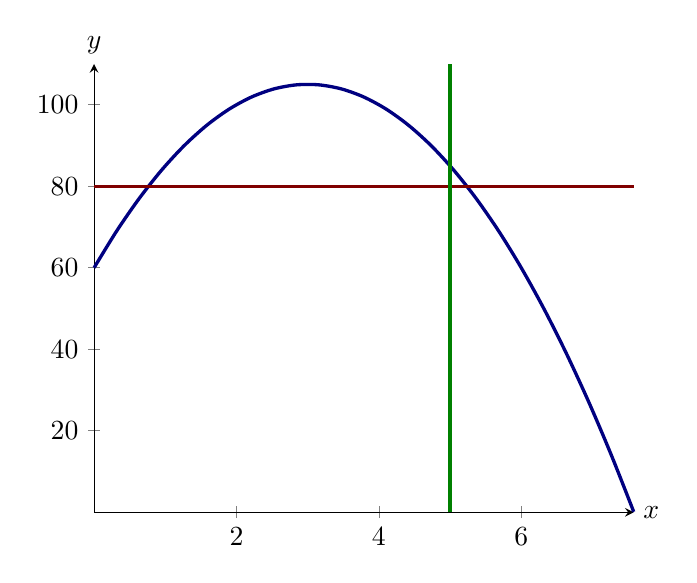
\begin{tikzpicture}
	\begin{axis}[
            clip=false, domain=0:7.58, axis lines =middle, xlabel=$x$,
            ylabel=$y$, every axis y label/.style={at=(current
              axis.above origin),anchor=south}, every axis x
            label/.style={at=(current axis.right of
              origin),anchor=west}, ]
          \addplot [very thick, penColor,smooth] {-5*x^2 +30*x+60};
          \addplot [very thick,penColor2] {80};
          \addplot [very thick, penColor4] plot coordinates {(5,0) (5,110)};
        \end{axis}
\end{tikzpicture}
\end{image}

As we have discussed, we can only find an inverse of a function when
it is one-to-one.  If a function is not one-to-one, but we still want
an inverse, we must restrict the domain. Let's see what this means in
our next examples.

\begin{question}
	Consider the graph of the function $f$ below:
	\begin{image}
          \begin{tikzpicture}
	    \begin{axis}[
	        ticks=none,
                domain=-2.5:2.5,
                width=6in,
                height=3in,
                xmin=-1.5, xmax=1.5,
                ymin=-1, ymax=1,
                axis lines =middle, xlabel=$x$, ylabel=$y$,
                every axis y label/.style={at=(current axis.above origin),anchor=south},
                every axis x label/.style={at=(current axis.right of origin),anchor=west},
              ]
              \addplot [very thick, penColor2, smooth, samples=100,domain=-2:2] {x^3-x-1/6};
              \node at (axis cs:1.3,1.5) [penColor2, anchor=west] {$f$};

              \addplot[color=penColor,fill=penColor,only marks,mark=*] coordinates{(-.9,0)};%%closed
              \addplot[color=penColor,fill=penColor,only marks,mark=*] coordinates{(-.58,0)};%%closed
              \addplot[color=penColor,fill=penColor,only marks,mark=*] coordinates{(-.17,0)};%%closed
              \addplot[color=penColor,fill=penColor,only marks,mark=*] coordinates{(.58,0)};%%closed
              \addplot[color=penColor,fill=penColor,only marks,mark=*] coordinates{(1.07,0)};%%closed          
              
	      \node at (axis cs:-1,-0.1) [penColor, anchor=west] {$A$};
              \node at (axis cs:-0.67,-0.1) [penColor, anchor=west] {$B$};
              \node at (axis cs:-0.33,-0.1) [penColor, anchor=west] {$C$};
              \node at (axis cs:0.47,-0.1) [penColor, anchor=west] {$D$};
              \node at (axis cs:1.03,-0.1) [penColor, anchor=west] {$E$};
              \node at (axis cs:1.15,0.6) [penColor2] {$f$};
            \end{axis}
          \end{tikzpicture}
        \end{image}
On which of the following intervals is $f$ one-to-one?
\begin{selectAll}
\choice[correct]{$[A,B]$}
\choice{$[A,C]$}
\choice[correct]{$[B,D]$}
\choice{$[C,E]$}
\choice[correct]{$[C,D]$}
\end{selectAll}
\end{question}

This idea of restricting the domain is critical for understanding
functions like $f(x) = \sqrt{x}$.

\begin{warning}
  We define $f(x) = \sqrt{x}$ to be the positive square-root, so that
  we can be sure that $f$ is a function. Thinking of the square-root
  as the inverse of the squaring function, we can see the issue a
  little more clearly.  There are two $x$-values that square to $9$.
  \[
  x^2 = 9\qquad\text{means $x=\pm 3$}
  \]
  Since we require that \textbf{square-root is a function}, we must
  have only one output value when we plug in $9$.  We choose the
  positive square-root, meaning that
  \[
  \sqrt{9}  =3.
  \]
\end{warning}


\begin{example}
  Consider the function
  \[
  f(x) = x^2.
  \]
  Does $f$ have an inverse? If so, what is it? If not, attempt to
  restrict the domain of $f$ and find an inverse on the restricted
  domain.
  \begin{explanation}
    In this case $f$ is not one-to-one. However, it is one-to-one on the
    interval $[0,\infty)$. Hence we can find an inverse of $f(x)=x^2$ on
      this interval. We plug $f^{-1}(x)$ into $f$ and write
      \begin{align*}
        f(f^{-1}(x)) &= \left(f^{-1}(x)\right)^2\\
        x &= \left(f^{-1}(x)\right)^2.
      \end{align*}
      Since the domain of $f$ is $[0, \infty)$, we know that $x$ is
        positive.  This means we can take the square-root of each side
        of the equation to find that
        \[
        \sqrt{x} = f^{-1}(x).
        \]
        \begin{image}
          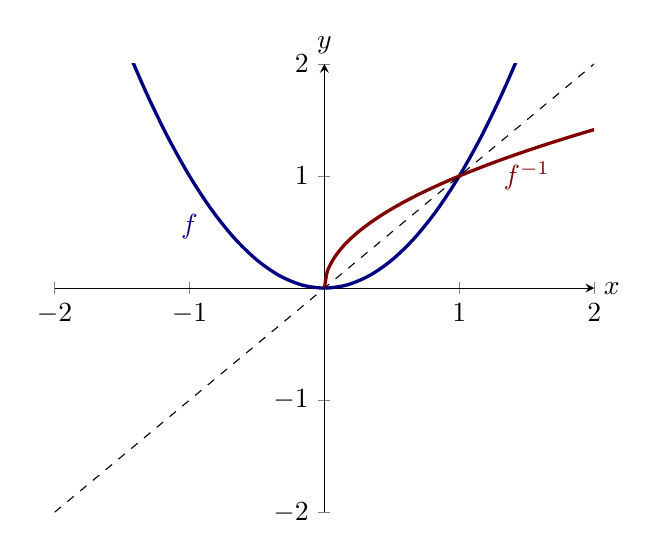
\begin{tikzpicture}
	    \begin{axis}[
            domain=-2:2,
            xmin=-2, xmax=2,
            ymin=-2, ymax=2,
            axis lines =middle, xlabel=$x$, ylabel=$y$,
            every axis y label/.style={at=(current axis.above origin),anchor=south},
            every axis x label/.style={at=(current axis.right of origin),anchor=west},
          ]
	  \addplot [very thick, penColor, smooth] {x^2};
          \addplot [very thick, penColor2, smooth, samples=100,domain=0:2] {sqrt(x)};
          \addplot [dashed, textColor] {x};
          \node at (axis cs:-1,.55) [penColor] {$f$};
          \node at (axis cs:1.5,1) [penColor2] {$f^{-1}$};
        \end{axis}
\end{tikzpicture}
%% \caption{A plot of $f(x)=x^2$ and $f^{-1}(x) = \sqrt{x}$. While
%%   $f(x)=x^2$ is not one-to-one on $\RR$, it is one-to-one on
%%   $[0,\infty)$.}
%% \label{plot:fxn and inverse x^2}
\end{image}
\end{explanation}
\end{example}



\begin{example}
Consider the function
\[
f(x) = x^3.
\]
Does $f(x)$ have an inverse? If so, what is it? If not, attempt to
restrict the domain of $f(x)$ and find an inverse on the restricted
domain.
\begin{explanation}
  In this case $f(x)$ is one-to-one. We may write
  \begin{align*}
    f(f^{-1}(x)) &= \left(f^{-1}(x)\right)^3\\
    x &= \left(f^{-1}(x)\right)^3\\
    \sqrt[3]{x} &= f^{-1}(x).
  \end{align*}
For your viewing pleasure we give a graph of $y=f(x)=x^3$ and
$y=f^{-1}(x)= \sqrt[3]{x}$. Note, the graph of $f^{-1}$ is the image
of $f$ after being flipped over the line $y=x$.
\begin{image}
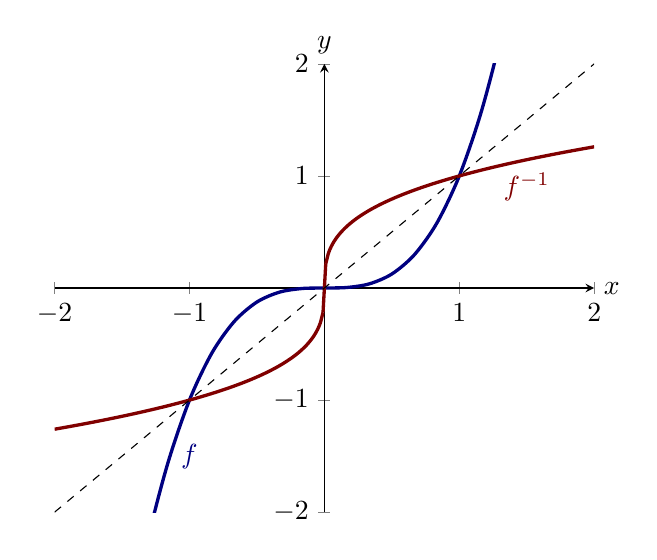
\begin{tikzpicture}
	\begin{axis}[
            domain=-2:2,
            xmin=-2, xmax=2,
            ymin=-2, ymax=2,
            axis lines =middle, xlabel=$x$, ylabel=$y$,
            every axis y label/.style={at=(current axis.above origin),anchor=south},
            every axis x label/.style={at=(current axis.right of origin),anchor=west},
          ]
	  \addplot [very thick, penColor, smooth] {x^3};
          \addplot [very thick, penColor2, smooth, samples=100,domain=.01:2] {x^(1/3)};
          \addplot [very thick, penColor2, smooth, samples=100,domain=-2:-.01] {-abs(x)^(1/3)};
          \addplot [very thick, penColor2] plot coordinates {(.01,.215) (-.01,-.215)};
          \addplot [dashed, textColor] {x};
          \node at (axis cs:-1,-1.5) [penColor] {$f$};
          \node at (axis cs:1.5,.9) [penColor2] {$f^{-1}$};
        \end{axis}
\end{tikzpicture}
%% \caption{A plot of $f(x)=x^3$ and $f^{-1}(x) = \sqrt[3]{x}$. Note
%%   $f^{-1}(x)$ is the image of $f(x)$ after being flipped over the line
%%   $y=x$.}
%% \label{plot:fxn and inverse x^3}
\end{image}
\end{explanation}
\end{example}




\end{document}

